%\clearpage
\chapter{Introduction}

%%%
\section{Shadow Removal}
%%%

\subsection{The Context}

Video analytics have seen a rise in popularity in many application fields, such as surveillance, data collection, and smart-city infrastructure. Some of these applications, e.g., the pedestrian and traffic counting seen in (Danner et al.'s) [\ref{Danner et al. ;) }], perform classification and analysis on moving objects. In order to detect and extract moving objects in an environment, foreground pixels are differentiated from those of the background through the use of statistical techniques, including Mixture of Gaussians, and Multi-Modal Mean [\ref{MoG}, \ref{MMM}]. These strategies establish a model of the background of a scene, which changes over time. This background model is then compared directly to a frame. By finding the difference between a frame and its background model, a mask containing the foreground pixels is created. Foreground pixels are then grouped together through the use of connected-component labeling, and segmented as a moving object. \hl{The moving object is then subjected to all sorts of analysis based on whatever the application needs.}

Applications that analyze moving objects rely on the accuracy of the extraction of foreground pixels. These applications are disadvantaged by the fact that shadows are often mischaracterized as foreground objects, and are included as part of a moving object. This is often due to shadows possessing similar movement patterns and brightness compared to non-shadow foreground objects [\ref{Sanin -> others}]. Figure \ref{fig:nonshadow} illustrates the effect shadows have on the segmentation of foreground objects. 

\begin{figure}
  \centering
  \begin{subfigure}{.49\linewidth}
  \centering
  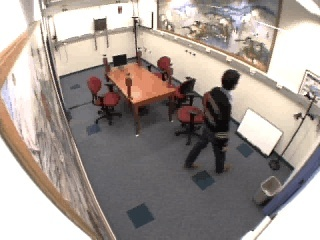
\includegraphics[width=1\linewidth]{figures/background/room_0295_frame.jpg}
  \end{subfigure}
  \hfill
  \begin{subfigure}{.49\linewidth}
  \centering
  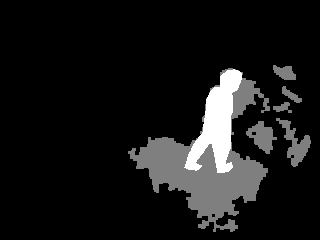
\includegraphics[width=1\linewidth]{figures/background/room_0295_shadows.jpg}
  \end{subfigure}
  \hfill
  \begin{subfigure}{.49\linewidth}
  \centering
    
\includegraphics[width=1\linewidth]{figures/background/room_0295_blob.jpg}
    \caption{}
  \end{subfigure}
  \hfill
  \begin{subfigure}{.49\linewidth}
  \centering
    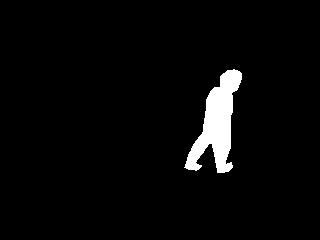
\includegraphics[width=1\linewidth]{figures/background/room_0295_clean.jpg}
    \caption{}
  \end{subfigure}
  \caption{(a) Improper segmentation of foreground objects. (b) With shadows removed, proper detection and tracking can be done on the moving object.}
\label{fig:nonshadow}
\end{figure}

The inclusion of shadows in foreground objects may hamper detection and tracking in several ways. Prominent issues, noted by Sanin et al. [\ref{Sanin}], include the distortion of an object's appearance model (required to properly track an object), and the erroneous joining of multiple objects into one labeled connected-component. Additional details regarding a shadow's effect on tracking can be found in [\ref{3,4 proposal?}]. The removal of shadows from foreground objects is thus a vital step in accurately segmenting moving foreground objects.

Classifying shadow pixels within moving foreground objects has been approached in numerous ways, including color-based attenuation models, geometric projective models, and texture-matching models [\ref{all these}, \ref{}, \ref{}]. Machine-learning has also been employed to attempt to learn the appearance of cast shadows in an unsupervised manner [\ref{Sato?}, \ref{Lee?}, \ref{Physical}]. A taxonomy of shadow removal methods produced by Prati et al. summarizes and evaluates four contemporary method classes: Statistical Nonparametric, Statistical Parametric, Deterministic Nonmodel-based and Deterministic Nonmodel-based 2 [2]. The study concluded that the simpler methods were more suited for general practice, but ``to detect shadows efficiently in one specific environment, [adding] more assumptions yield better results.'' A second algorithm survey conducted by Sanin et al. in [1] evaluated more modern methods (catalogued as Chromacity, Geometry, Physical, Small Region Texture, and their own contribution, Large Region Texture) on the same datasets as above, yielding similar results concerning the generalization of shadow removal to an arbitrary scene. Mitra et al. provides a survey of threshold selection strategies for identifying shadows in moving foreground objects [3].

\subsection{The Problem}

The surveys indicate that the surveyed shadow removal algorithms fail to optimally adapt to various environmental properties; these methods quantifiably benefit from assumptions made about key factors of a scene, including illumination constancy, color content, and shadow intensity. In order to facilitate optimization, shadow removal methods (surveyed by Sanin et al.) possess algorithm parameters that are manually tuned to an environment. The reliance on environmental assumptions affects shadow removal in two ways: firstly, shadow removal performs suboptimally when deployed in an arbitrary environment, and secondly, even when manually calibrated, shadow removal fails to adapt to environmental parameters that change over time. From an application context, a surveillance system that monitors an sun-lit environment 24 hours a day will possess a wide range of shadow qualities when comparing shadows cast at dawn to shadows cast in the evening. Shadows cast in the same location may vary in darkness, size, orientation, and shape depending on the time of day. The indicates the need for shadow removal to adapt not only to diverse environments, but continually adapt as environmental properties vary over time.

We quantitatively demonstrate several cases that indicate the need for adaptation. Shadow removal is judged by its detection rate and its discrimination rate, further detailed in section \ref{section:eval_metrics}. Detection rate indicates the number of shadow pixels correctly identified, while discrimination rate indicates the number of foreground object pixels are correctly identified. Figure \ref{fig:vthreshdefault} modifies a parameter belonging to Large-Region Texture (LRT) shadow removal, which controls the chromacity range a shadow can lie in. Frames from the datasets CAVIAR and ATON (detailed in section \ref{section:datasets}) [\ref{caviar}, \ref{aton}]. The parameter (\textit{vThreshLower}) causes LRT shadow removal to perform optimally in the CAVIAR frame at its default value, 121. Similarly, the same algorithm performs poorly in the included dataset aton\_highway1 with the default parameters. However, if \textit{vThreshLower} is modified from 121 to 15, CAVIAR experiences a 47\% loss of discrimination, while aton\_highway1 gains 85\% detection in exchange for a 13\% loss of discrimination. Geometry shadow removal was found to also showcase different results on the same scene, but with differing parameters (Figure \ref{fig:gweight}). 
%Figure \ref{fig:vthreshdefault}, Figure \ref{fig:vthresh15} and Figure \ref{fig:gweight} demonstrate the necessity for parameter adaptation to occur between environments.

%\begin{figure}
%  \centering
%  \begin{subfigure}{.45\linewidth}
%    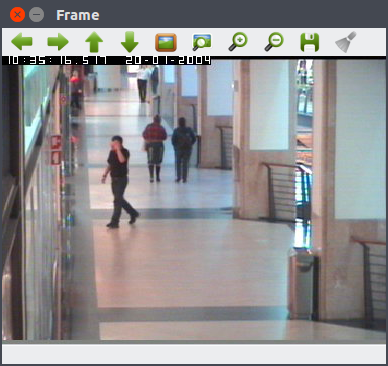
\includegraphics[width=1\linewidth]{figures/background/frame_caviar.png}
%    \caption{CAVIAR}
%  \end{subfigure}
%  \hfill
%  \begin{subfigure}{.49\linewidth}
%    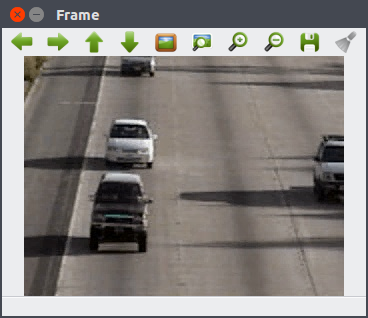
\includegraphics[width=1\linewidth]{figures/background/frame_highway1.png}
%    \caption{aton\_highway1}
%  \end{subfigure}
%  \caption{Original dataset frames.}
%\end{figure}

% vthresh default
\begin{figure}
  \centering
  \begin{subfigure}{.48\linewidth}
    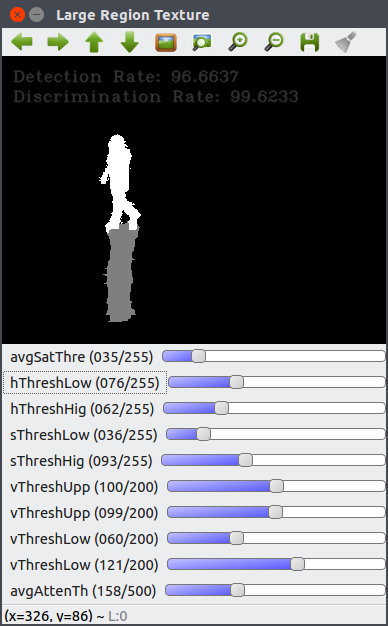
\includegraphics[width=1\linewidth]{figures/background/lr_caviar_default.png}
    \caption{}
  \end{subfigure}
  \hfill
  \begin{subfigure}{.49\linewidth}
    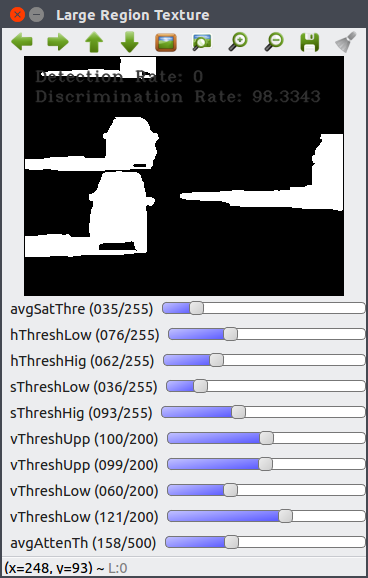
\includegraphics[width=1\linewidth]{figures/background/lr_highway1_default.png}
    \caption{}
  \end{subfigure}
  \caption{Default parameters (Datasets provided by Sanin, et al. [\ref{Sanin}]) (a) Detection: 96.6637, Discrimination: 99.6233. (b) Detection: 0, Discrimination: 98.3343}
  \label{fig:vthreshdefault}
\end{figure}

% vthresh15
\begin{figure}
  \centering
  \begin{subfigure}{.48\linewidth}
    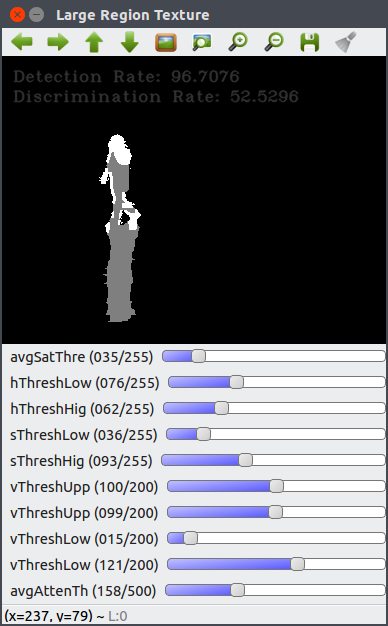
\includegraphics[width=1\linewidth]{figures/background/lr_caviar_thresh15.png}
    \caption{\textit{vThreshLower: 121}}
  \end{subfigure}
  \hfill
  \begin{subfigure}{.49\linewidth}
    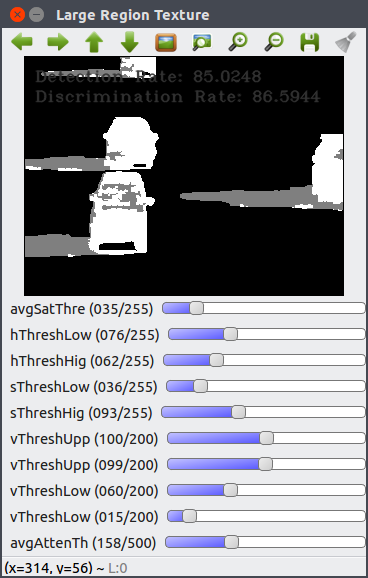
\includegraphics[width=1\linewidth]{figures/background/lr_highway1_thresh15.png}
    \caption{\textit{vThreshLower: 15}}
  \end{subfigure}
  \caption{\textit{vThreshLower} shifted from '121' to '15.' (Datasets provided by Sanin, et al. [\ref{Sanin}]) (a) Detection: 96.7076, Discrimination: 52.5296. (b) Detection: 85.0248, Discrimination: 86.5944}
  \label{fig:vthresh15}
\end{figure}

% gweight
\begin{figure}
  \centering
  \begin{subfigure}{.49\linewidth}
    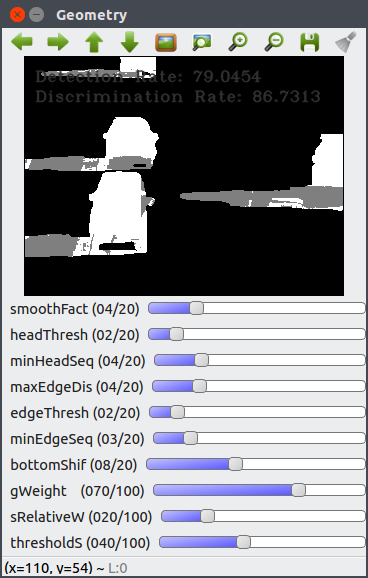
\includegraphics[width=1\linewidth]{figures/background/geo_highway1_default.png}
    \caption{\textit{gWeight: 70}}
  \end{subfigure}
  \hfill
  \begin{subfigure}{.49\linewidth}
    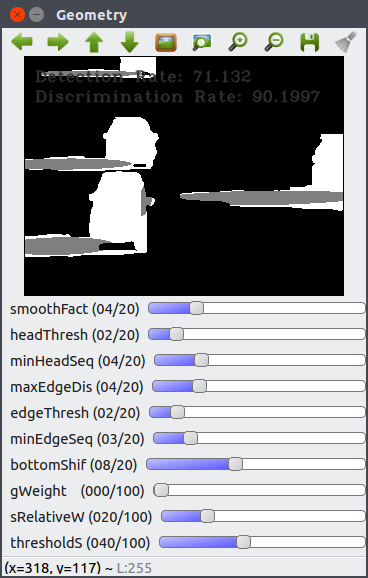
\includegraphics[width=1\linewidth]{figures/background/geo_lower_gweight.png}
    \caption{\textit{gWeight: 0}}
  \end{subfigure}
  \caption{\textit{gWeight} shifted from '70' to '0.' (a) Detection: 79.0454, Discrimination: 86.7313. (b) Detection: 71.132, Discrimination: 90.1997}
  \label{fig:gweight}
\end{figure}



%Precedent exists for intelligently adapting parameters for shadow removal. Sanin et al., in the implementation of Large Region Texture shadow removal, measure the average global attenuation, saturation, and foreground object perimeter of a scene. The algorithm selects several differing parameter values for hue, saturation, and value thresholds based on the average shadow attenuation and saturation of the scene. It also modifies the texture differential radius needed to qualify a pixel as shadow based on the perimeter of the foreground object in question. Our research seeks to provide a fully scalable approach, however, as the thresholds established for switching between parameter sets remain empirically determined and coarse-grained.

%%%

\FloatBarrier
\section{Objective and Contributions}

%None of the shadow removal methods analyzed are robust enough to compensate for environmental changes over time, nor do they optimally perform in an environment without a priori calibration of algorithm parameters. 
Our research seeks to establish an understanding of environmental properties that affect shadow removal, and utilize that understanding to optimize shadow removal in an arbitrary environment. This is achieved by automatically calibrating an algorithm's parameters based on observed environmental properties. Furthermore, we seek to create an understanding of how these environmental properties change over time, in order to continuously adapt shadow removal algorithms. These objectives require the creation of an adaptive model which automatically configures a shadow removal method to optimally perform given the observed environmental properties.

Our research makes multiple contributions \textit{how do I phrase this...?}. (We perform a qualitative assessment of each algorithm's performance in various environments.) We construct and utilize a framework for evaluating the sensitivity of an algorithm in regards to its mutable parameters. We identify and quantify observed environmental properties, and correlate them to sensitive algorithm parameters. Finally, we demonstrate the construction of an adaptive model, capable of leveraging correlated environmental properties to automatically tune an algorithm's parameters. The demonstration is completed by constructing a proof-of-concept model for Physical shadow removal using its parameter \textit{coneR1}.

Our proof-of-concept adaptive model draws upon the correlation between brightness attenuation in shadow regions and \textit{coneR1}, and improves shadow detection by up to 10\% and shadow discrimination by up to 28\%. Additional indirect environmental factors are found to modify the effectiveness of the adaptive model. Various brightness calculation methods are shown to influence attenuation correlation by 7\% to 20\%.
A study of low-contrast feature keypoints in a scene was shown to occasionally improve attenuation-correlation by up to 12\%.

In Chapter 2, we detail the shadow removal algorithms utilized in this study, and outline the steps taken to produce an adaptive model. Chapter 3 assesses the shadow removal algorithms for their performance in diverse environments, as well as their sensitivity to parametric change. These assessments culminate in the construction of a proof-of-concept adaptive model for Physical shadow removal, using its \textit{coneR1} parameter. Chapter 3 also explores indirect environmental properties and their potential impacts on the performance of the adaptive model. Chapter 4 quantifies and discusses the results of the adaptive model, and the indirect environmental properties' effects on the model. Chapter 5 concludes with analysis and future work. 

%Characterization of a scene or environment is traditionally done with global parameters such as global hue, saturation, and value (HSV), or color variance. However, more scene properties are needed for proper identification of semantic scene content, needed for this	 research. The ‘gist’ of scene, proposed by Oliva et al. in [5], compares evaluations of the properties of scene, using low-level features and simple arrangement of volumetric forms. Similarly, in [6], Oliva et al. evaluates the content of a scene using shape modeling such as the openness, ruggedness, roughness, expansion of a scene, creating the ‘spatial envelope’ of a scene. Lowe et al. propose the scale-invariant feature transform (SIFT), which utilizes and identifies features of a scene that are robust to noise, illumination, distortion, and viewpoint [7]. Bayesian Scene Modeling, proposed by Fei-Fei et al., utilizes the ‘bag-of-words’ strategy, building a dictionary of codewords relevant to a scene via unsupervised machine learning [8]. This approach creates a ‘theme’ for a scene built upon these collected codewords, categorizing complex diverse scenes into 13 categories (highway, coast, mountain, etc). 

%There is precedent for intelligently adapting parameters for shadow removal. Sanin et al., in the implementation of Large Region Texture shadow removal, measure the average global attenuation, saturation, and foreground object perimeter of a scene. The algorithm selects several differing parameter values for hue, saturation, and value thresholds based on the average shadow attenuation and saturation of the scene. It also modifies the texture differential radius needed to qualify a pixel as shadow based on the perimeter of the foreground object in question.

%\section{Work Completed}

%The implementations of the various approaches came with hard-coded parameters that were found to be correspondent with the provided datasets. Prominent parameters include:

%There are many more mutable parameters that affect shadow removal efficacy, and again, a more complete taxonomy will be provided. 
%In order to then quickly evaluate the effect of modifying these in-built parameters, a graphical interface was created to adjust them during runtime and view the effects. The interface supports either entire sequences (e.g. video) or singular frames. The interface supports any of the aforementioned shadow removal methods. 

%Fig. 1. Graphical interface for permuting parameters.

%The graphical interface is a crucial development in terms precisely measuring each parameter's effect on a given scene. However, in order to study shadow removal in terms of adaptivity over time, a more procedural method was required. Courtesy of username ‘brofield’, SimpleINI (github.com/brofield/simpleini), licensed under MIT, allowed for creation of .ini files containing any given removal method's default parameters. The algorithms themselves were then modified to allow for runtime modifications to be made to these parameters, meaning a procedural, iterative approach to analysis was created. A python script capable of writing to this .ini file allows for rapid permutation of parameters and values.

%Develop holistic scene content understanding in order to select shadow removal method for the ‘macro’ stage of hypervisor program. A quantization of seemingly qualitative scene content is required to better select between shadow removal methods. Some of this scene content includes shadow orientation vs. foreground object orientation, pre-existing static scene shadows, foreground object classification, distinctiveness of foreground objects (color differences in particular), light source in a scene, and many more. Building up an understanding of these scene properties may also help with the ‘micro’ stage of the proposed framework.

%Develop understanding of how these scene/environment parameters change over time of day and between locales. Observation of how both the quantitative and qualitative scene parameters change over time is required to create the proposed adaptive framework. This step will be simple for things like shadow intensity and global saturation, but more difficult for aforementioned properties like static shadows and object classification.

%Create correlation between global scene/environment properties and shadow removal accuracy. This step represents the main experimental thrust of the proposed research detailed thoroughly in this research summary.

%Use the aforementioned correlation to build hypervisor program to deploy adaptive shadow removal in arbitrary scenes and environments. This will be done primarily in C++, using the OpenCV API.
